\documentclass[deutsch]{lib/llncs/llncs}
\usepackage{lib/llncs/llncsdoc}
\usepackage[ngerman]{babel}
\usepackage[utf8]{inputenc}
\usepackage{hyperref}
\usepackage{graphicx}
\usepackage{lib/picins/picins}
\usepackage[nottoc]{tocbibind}


\begin{document}
\markboth
{Anwendung des ''Technology Acceptance Model'' zur Akzeptanzbestimmung qualifizierter elektronischer  Fernsignaturen im Unternehmensumfeld}
{Anwendung des ''Technology Acceptance Model'' zur Akzeptanzbestimmung qualifizierter elektronischer  Fernsignaturen im Unternehmensumfeld}
\thispagestyle{empty}


\begin{flushleft}
\LARGE\bfseries Anwendung des ''Technology Acceptance Model'' zur Akzeptanzbestimmung qualifizierter elektronischer  Fernsignaturen im Unternehmensumfeld


\end{flushleft}
\rule{\textwidth}{1pt}
\vspace{2pt}


\begin{flushright}
\Huge


\begin{tabular}{@{}l}
Interdisziplinäre und \\
sozialwissenschaftliche \\
Reflexion der Informatik 2\\\\
Wintersemester 2017/2018\\\\
Frank Dreyer\\
Matrikelnummer: 741827\\\\
07.02.2018\\[6pt]
\end{tabular}


\end{flushright}
\rule{\textwidth}{1pt}
\vfill

\newpage
\tableofcontents
\newpage\vspace{2pt}


\section{Grundlagen}


\subsection{Technology Acceptance Model}
Das \textit{Technology Acceptance Model} \cite{Zitat01}, kurz TAM, ist ein von von Fred D. Davis entwickeltes Akzeptanzmodell, welches auf dem sozialpsychologischem Modell \textit{Theory of Reasond Action} (TRA) von Ajzen und Fishbein \cite{Zitat04} basiert. Das Modell zielt darauf ab, Erkenntnisse darüber zu gewinnen, ob und warum Personen Technologien akzeptieren oder diese ablehnen. \\
Dabei wird angenommen, dass eine Person mit positiver Nutzungseinstellung zur Technologie diese auch tatsächlich verwendet. (Vgl. \cite[p. 237]{Zitat03}) Diese Nutzungseinstellung hängt wiederum maßgeblich von den Faktoren 'wahrgenommener Nutzen' und 'wahrgenommener Bedienungskomfort' ab. \\
Der 'wahrgenommene Nutzen' beschreibt das subjektiv Empfinden, dass sich eine Technologie positiv auf die Steigerung der eigenen Arbeitsleistung in einem organisatorischem Kontext auswirkt.  (Vgl. \cite[p. 320]{Zitat02}) \\
Der 'wahrgenommene Bedienungskomfort' bezeichnet das subjektive Empfinden, dass die Verwendung einer Technologie mit wenig Aufwand verbunden ist, bzw. dass die Technologie einfach zu benutzen ist. (Vgl. \cite[p. 320]{Zitat02}) \\
Bandow und Holzmüller fassen die Auswirkung dieser beiden Determinanten folgendermaßen zusammen: ''Je größer der Nutzen eines Informationssystems und je einfacher dessen Bedienbarkeit, desto eher ist der Anwender dazu bereit, das neue System zu nutzen.'' (Vgl. \cite[p. 237]{Zitat03}) \\
Auf den 'wahrgenommenen Nutzen', wie auch den 'wahrgenommenen Bedienungskomfort' wirken wiederum 'externe Variablen', die unter anderem demografische und persönliche Merkmale des Akteurs umfassen, im Originalmodell allerdings nicht weiter spezifiziert werden. (Vgl. \cite[p. 21]{Zitat01}) \\
Abbildung 1 illustriert das Modell.
\begin{figure}
	\centering
	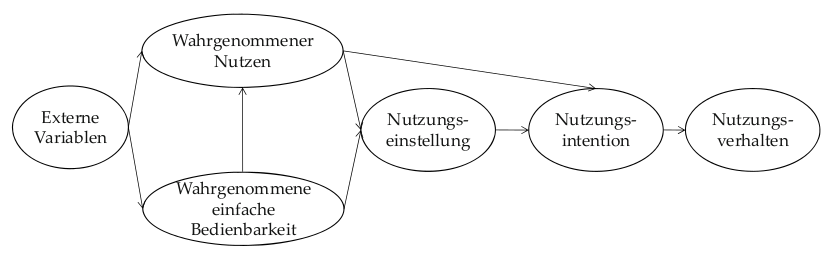
\includegraphics[scale=0.40]{img/abbildung1.png}
	\caption{\textit{Technology Acceptance Model} (Vgl. \cite[p. 237]{Zitat03})}
\end{figure}


\subsection{Digitale Signaturen}
Digitale Signaturen sind in Grenzen vergleichbar mit konventionellen Unterschriften auf Papier, welche über ein asymmetrisches kryptographisches Verfahren digitalisiert wurden. (Vgl. \cite[p. 297]{Zitat06}) Dieses asymmetrische Kryptosystem schließt drei Prozesse mit ein: den 'Unterschriftsprozess', den 'Authentifizierungsprozess' sowie den 'Prozess zur Sicherung der Datenintegrität'. (Vgl. \cite[p. 4]{Zitat05}) \\
Beim 'Unterschriftsprozess', muss sich die Person, die das jeweilige Dokument unterzeichnen soll, zunächst identifizieren. Die Identifikation hängt von der Implementierung ab und kann dementsprechend unter anderem über eine PIN, ein Passwort oder auch einen sequenz-basierten Token-Code abgewickelt werden. Ist die Identität des Unterzeichners bestätigt, so erhält er ein Zertifikat mit seiner Identität und einem öffentlichem und privatem Schlüsselpaar, mit dem er das Dokument signieren kann. Dafür wird zunächst ein einzigartiger mathematischer Code aus dem Dokument generiert, der im Anschluss über den privaten Schlüssel verschlüsselt, bzw. ''signiert'', wird. Um den 'Unterschriftsprozess' abzuschließen wird das Dokument zusammen mit der Signatur (dem verschlüsseltem mathematischen Code) an den Empfänger gesandt. (Vgl. \cite[p. 4]{Zitat05}) \\
Der Empfänger kann daraufhin im 'Authentifizierungsprozess' überprüfen, ob das Dokument auch von der richtigen Person unterzeichnet wurde. Dafür fordert er den öffentlichen Schlüssel der Unterzeichners an und kann daraufhin mit dem öffentlichen Schlüssel den mathematischen Code entschlüsseln. Das Entschlüsseln wird nur dann funktionieren, wenn das Dokument mit dem korrespondierenden privaten Schlüssel verschlüsselt wurde und kann daraus folgernd auch die Authentizität garantieren. (Vgl. \cite[p. 4]{Zitat05}) \\
Zum Schluss wird im 'Prozess zur Sicherung der Datenintegrität' überprüft, ob das Dokument nach dem Signieren nicht mehr verändert wurde. Dafür wird erneut der mathematische Code aus dem Dokument generiert und mit dem im 'Authentifizierungsprozess' entschlüsselten mathematischen Code verglichen. Beide müssen identisch sein um sicher zu sein, dass das Dokument nach dem Unterschreiben nicht modifiziert wurde.  (Vgl. \cite[p. 4]{Zitat05})


\bibliographystyle{amsalpha}
\bibliography{lit/lit}


\end{document}
